\section{Scanner Flow}

\subsection{Overview}
Here we discuss the systems that must be built for vaccine clinics and distributors in order to enable the use of the SafePaths card framework presented above. We present several relevant protocols as well as the functionality of a proposed vaccine distributor/verifier scanner app. This scanner app would be necessary to function with the encrypted QR codes described above. 

\subsection{Vaccine eligibility confirmation}
Phased vaccination using the SafePaths card system requires the distribution of SafePaths cards containing digitally signed \textit{Coupons} to appropriate subsets of the population during each stage of vaccination. There are several ways that this might be achieved. We propose potential solutions below, though we recognize that these strategies must be determined by individual jurisdictions to meet the circumstances in different locations.  


\begin{enumerate}
    \item Disseminate to businesses to provide to employees (eg: hospitals, restaurants, etc. as appropriate)
    \item Make available at local government building (similar to DMV process of obtaining a driver’s license)
    \item Mail out to individuals based on employment/other factors (via background check systems, centralized databases such as IRS) 
\end{enumerate}


\begin{figure}[!ht]
\begin{center}
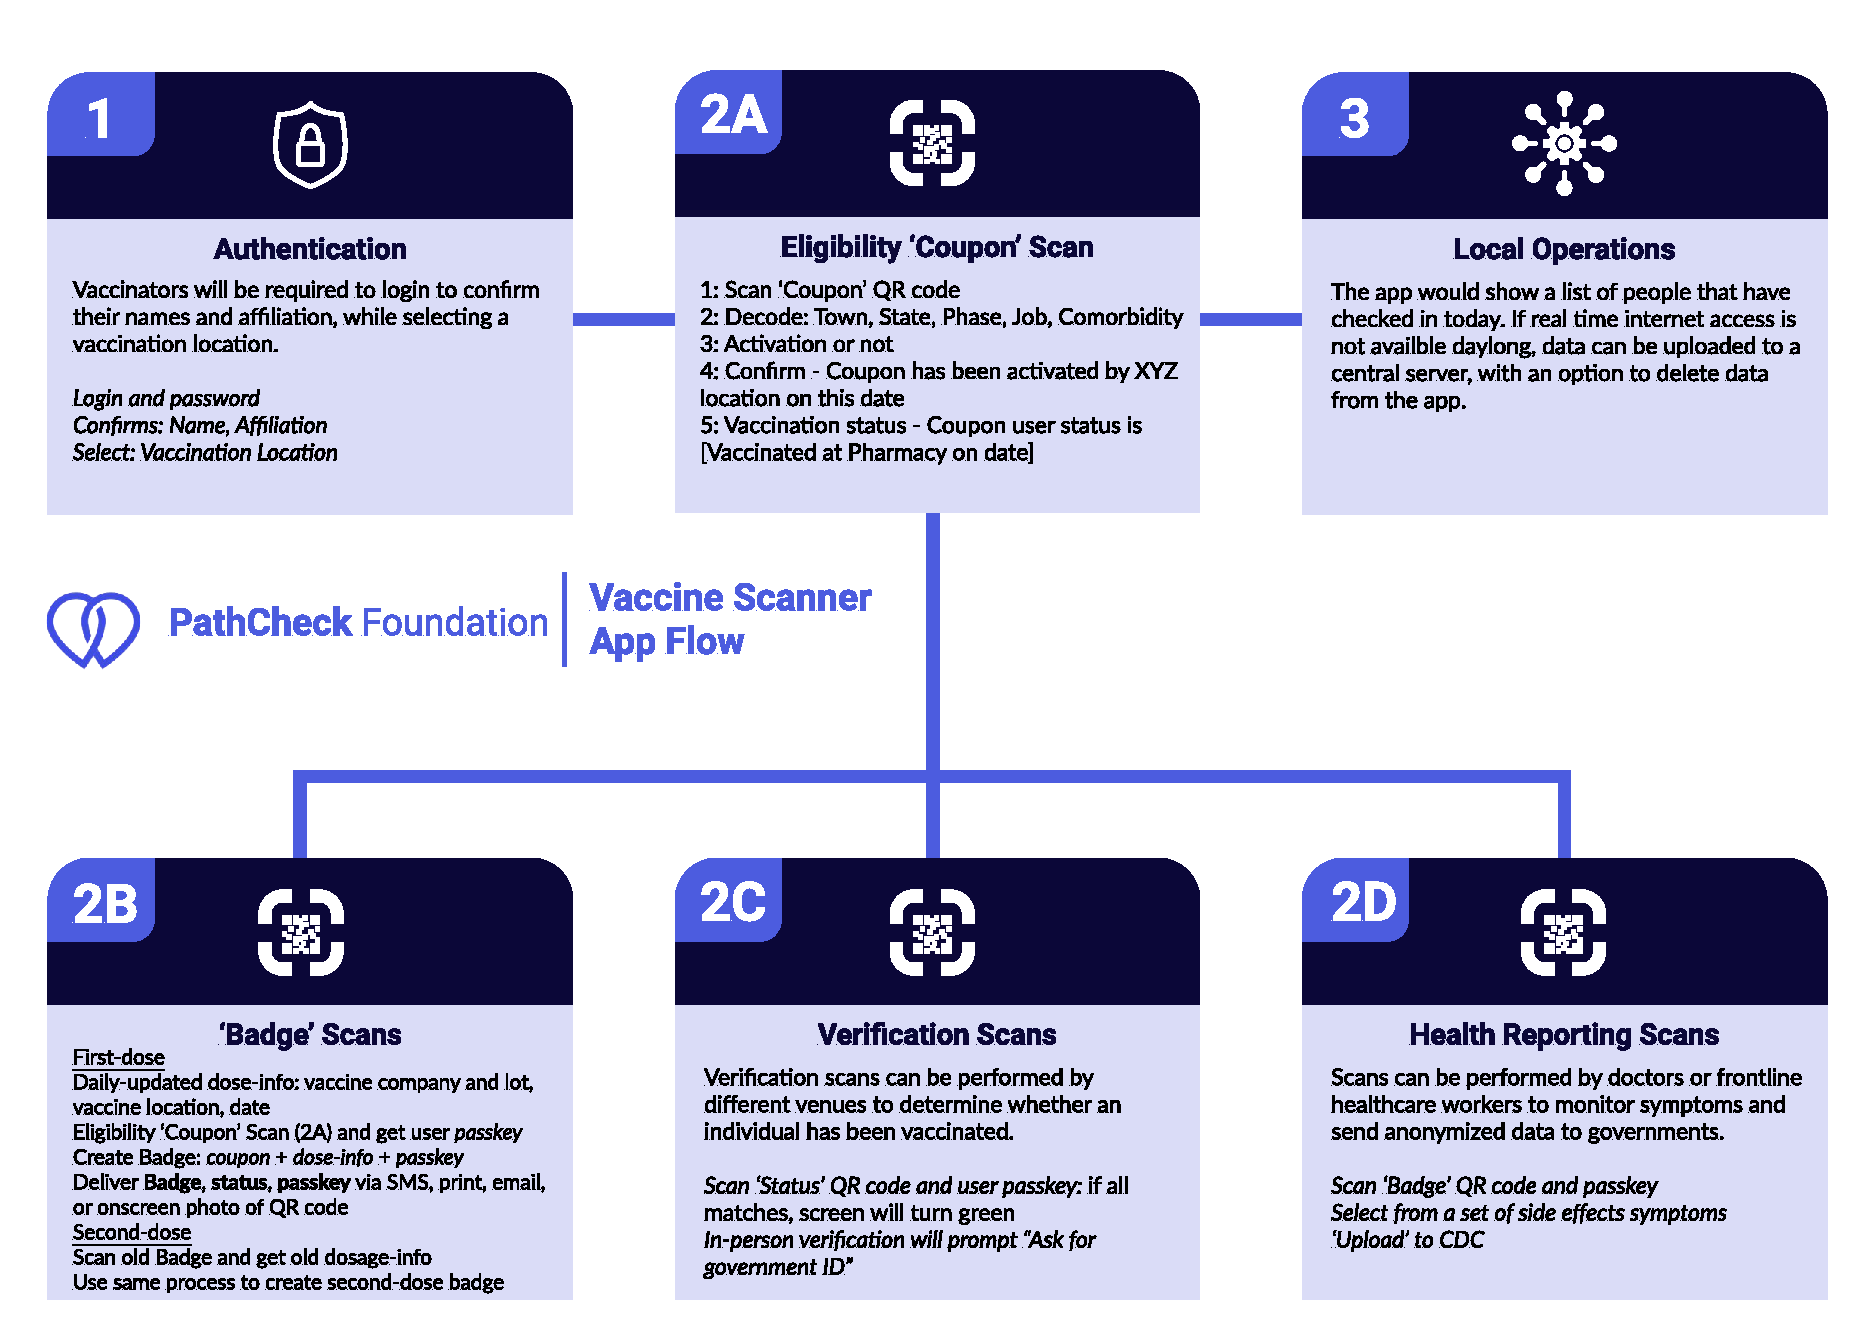
\includegraphics[width=13.5cm]{images/scanner_protocol.pdf}
\end{center}
\caption{Scanner app protocol workflow diagram.}
\label{scanner-workflow}
\end{figure}


\subsection{Vaccine administration}
To confirm an individual for vaccination scheduling/check-in, a clinic must verify the authenticity of a vaccine recipient’s QR \textit{Coupons}. The first function of our proposed scanner app would be to scan a vaccine recipient’s \textit{Coupon} to determine authenticity and prevent the use of a single \textit{Coupon} by multiple individuals. This would be achieved by scanning the digital signature present on a SafePaths \textit{Coupon} and verifying its digital signature. 

The second function of our proposed scanner app would be to create digitally signed \textit{Badge} and \textit{Passkey} stickers for post vaccination. This would make use of our previously described algorithm (\cite{crypt}) for secure recording of vaccine information into a \textit{Badge} sticker, encrypted using the encryption key present in the \textit{Passkey}. After creating these stickers, the proposed scanner app would not store any information regarding a recipient’s encryption key; that information would only exist within the \textit{Passkey} sticker. 

\subsection{Second dose}

Second dose administration functionality would be implemented into the scanner app in the same manner as described in the previous section for ‘Vaccine Administration’. A \textit{Status} sticker would be created by the scanner app in a similar manner to the \textit{Badge} sticker, also drawing on the methods described in our cryptographic protocol (\cite{crypt}). 

\subsection{Record-keeping}
Another critical function of our scanner app would be the ability to integrate with existing systems, such as VAMS in the United States. Ideally, our app would be able to automatically provide vaccination record information to VAMS while replacing PII with pseudo identifiers. 

Alternatively, our scanner system would also have the capability to directly aggregate vaccination record data in an anonymized fashion, retaining population-level statistics such as vaccination prevalence in a given jurisdiction that might be important for public health policy development. Details concerning clinic location, vaccine dose, and vaccine manufacturer could be stored by the scanner app and aggregated for public health official viewing.  


\subsection{Vaccination verification}
Our proposed scanner app would enable vaccination verification simply by reading immunization status contained in a user’s \textit{Status} sticker. For further identity verification, a form of ID (such as driver’s license) can be compared with the decrypted PII from the scanner app using an individual’s \textit{Passkey} sticker.  The scanner app would not store this information following completion of the immunization confirmation.

